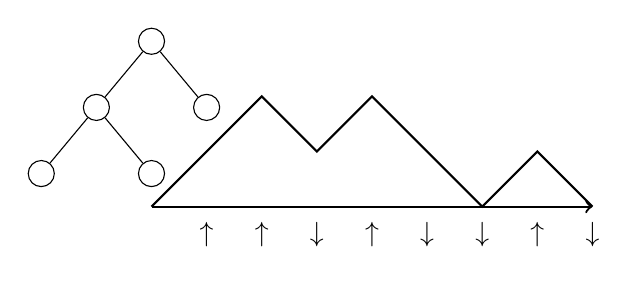
\begin{tikzpicture}[scale=0.7,level distance=1.2cm,sibling distance=2cm]
  % Arbre binaire
  \node[circle,draw] (root) {} child { node[circle,draw] (left) {} child { node[circle,draw]
      {} } child { node[circle,draw] {} } } child { node[circle,draw] (right) {} };

  % Chemin de Dyck correspondant
  \draw[->,thick] (0,-3) -- (8,-3); \draw[thick] (0,-3) -- (1,-2) -- (2,-1) -- (3,-2) --
  (4,-1) -- (5,-2) -- (6,-3) -- (7,-2) -- (8,-3);

  % Labels des montées et descentes
  \node at (1,-3.5) {\(\uparrow\)}; \node at (2,-3.5) {\(\uparrow\)}; \node at (3,-3.5)
  {\(\downarrow\)}; \node at (4,-3.5) {\(\uparrow\)}; \node at (5,-3.5) {\(\downarrow\)};
  \node at (6,-3.5) {\(\downarrow\)}; \node at (7,-3.5) {\(\uparrow\)}; \node at (8,-3.5)
  {\(\downarrow\)};
\end{tikzpicture}
